\section{\label{sec:level1}Two-Dimensional Time}

According to many spiritual traditions, including those that rely on
direct observation through meditation, the consciousness of humans, animals,
and all living things is a combination of the finite and the infinite,
existing both inside and outside of time.
Allowing more than one dimension of time may support this view
of life beyond the supposed material world.
The existence of non-local mind effects, since they hold up under serious
investigation \cite{Kelly}, provides an impetus for the investigation of
multi-dimensional time as an aspect of consciousness.

The Wheeler-DeWitt equation \cite{DeWitt} attempts to combine mathematically
the ideas of quantum mechanics and general relativity.
One of its implications is the ``problem of time'',
which is a conceptual conflict between general relativity (GR)
and quantum mechanics (QM).
Quantum mechanics regards the flow of time as universal and absolute, whereas
general relativity regards the flow of time as malleable and relative.

According to Wheeler-DeWitt, an observer outside of the universe
doesn't experience time. Page and Wootters \cite{Page} addressed this paradox
(time \textit{seems} real enough) by treating time as an emergent phenomenon
resulting from quantum entanglement.
Experiments \cite{Moreva} on entangled particles have bolstered the theory.

There are other takes on timeless universe models.
Aharonov's two-state formalism of quantum mechanics has also been used
\cite{Lobo} to propose emergence of time from a timeless unus mundus
quantum-like space.
Jianfeng Li provides a good overview \cite{Jianfeng} of quantum mechanical
timeless consciousness.
Ralph Abraham and Sisir Roy \cite{AbrahamRoy} have proposed a
mathematical model for the quantum vacuum as a model of consciousness.
In it, spacetime emerges from the subtle $akasha$
existing outside of space and time. 

There are two distinct types of time: emergent time, which emanates from the
structure of space-time and its metrics, and a causal time, indicating the flow
from the past to the future \cite{Brunet}. The time domains relate the
two models of Physics: QM and GR. 
Note that since quantum mechanical effects can happen in either time direction,
emergent time could just as well flow from the future to the past.

In the interest of having a nomenclature for this paper, one dimension of time
is the ``quantum time'' domain and the other is the ``relative time'' domain.
So, \textit{quantum time} and \textit{relative time}.

The word \textit{quantum} is used in the Bohmian sense.
The Bohmian interpretation of quantum mechanics is non-local.
Experiments in non-locality \cite{Achterberg} find that the mind extends beyond
the skull. 

To please the poets, let's put an Eastern spin on these 
well-established fields:

\begin{itemize}
  \item GR = Yang: Time is space
  \item QM = Yin: Time is consciousness
\end{itemize}

\subsection{Quantum Time and Consciousness}

In the field of ``quantum biology'',
there are many examples of biological systems exploiting quantum effects.
One could suppose that nature would evolve to use quantum time.

The physical vacuum, a substrate for quantum interactions,
is a natural mechanism for biological systems to have evolved to utilize.
This pantheistic view allows for consciousness as the ground state of being.
Consciousness is the interaction between the physical vacuum and biology which
facilitates communication at any physical scale, from DNA to species.

This provides a possible signaling mechanism for consciousness in beings such
as paramecia or slime molds, which exhibit conscious behavior but are too small
for consciousness to arise from the network effects of neurons or ganglia.

The mechanics of signal generation can be considered in the context of
quantum time.
This arrangement lends itself to information flow, utilized by nature,
between the time and timeless domains.

Resonance is treated as a physical phenomenon occurring in quantum time $\tau$.
A resonant frequency in $\tau$ is equivalent to a frequency chirp in $t$.
This dynamic emergence of time should produce small but detectable artifacts.
The stream of consciousness is treated as emerging from a probabilistic field
rather than time abruptly appearing from nothing.

Biological systems evolve to minimize the expenditure of energy. Resonances
(field analogs of electrical and mechanical ringing) require a small energy
input to keep them going, assuming a reasonably high Q. It stands to reason
that biological systems would use field resonances in the physical vacuum
(the exact nature of the field doesn't need to be understood)
to transmit consciousness information efficiently.

In other words, there is a basis for the belief that ``It's all vibrations''
if the vibrations occur in quantum time such that their signal artifacts
produce what looks like a noise spectrum.
This is almost certainly an overly simplified view,
but perhaps sufficient to reach low-hanging fruit.
There could be other time dimensions at play or
even backward time effects providing the excitation for the resonance.
Since we're only looking for artifacts, the details aren't as important
as verifying the existence of the artifacts in the first place.

We live in a world of electronic noise, much of which is not fully understood.
By digitizing and processing this noise in warped time domains,
consciousness information could conceivably be extracted from the
resulting signals using traditional detection technologies.

\subsection{Relating Time Domains by Exponential}

One way to relate the two time dimensions is with a scale-invariant geometry
that exploits self-similarity.
For it to be scale-invariant,
we use an exponential growth model for quantum time.

\begin{equation} \label{eq:pink}
\tau \propto e^{\epsilon t}
\end{equation}

This power law relationship between $\tau$ and $t$
is a key enabler of signal transformations.
A sample test signal with ``warp factor'' $\omega$ for Eq. \ref{eq:pink} is:
\begin{equation} \label{eq:wp}
Signal \propto sin(k \cdot e^{\omega t})
\end{equation}
The superposition of exponential chirps is also pink.
Since it's self-similar,
overlapped versions can be correlated for more processing gain.
Reversing $\tau$ and $t$ in Eq. \ref{eq:pink} gives:

\begin{equation} \label{eq:brown}
t \propto e^{\epsilon \tau}
\end{equation}

Which seems like a good idea,
but the time domain chirp is then no longer a power function.
Overlapping transforms in time doesn't work, limiting its utility.
It's logarithmic, which is not self-similar.
A test chirp for Eq. \ref{eq:brown} is:

\begin{equation} \label{eq:wb}
Signal \propto sin(k \cdot log^{\omega t + 1})
\end{equation}

Returning to Eq. \ref{eq:pink}, the implication seems to be that relative time
emerges from quantum time. It could be likened to a lake being filled by rain.

\subsection{Relating Time Domains by Conic Section}

Consider the case where $\omega$ in Eq. \ref{eq:wp} is imaginary.
The chirp frequency follows a cosine function (see Euler's Formula).
Supposing the existence of a high frequency pilot tone $f_0 \gg F_S/2$ mixing
with the chirp, the resulting frequency would follow approximate a
parabolic path down to 0 and back up again.

The parabolic model allows independence from the arrow of time since $x^2$ is
symmetric in $x$. You would expect such independence in quantum time.
A $\tau/t$ singularity occurs at ``the now'' in Eq. \ref{eq:parabolic},
which I call ``the dharma point'' because it merges with eternity.
With an amplitude that goes as $\sqrt{|t - t_{now}|}$, the spectrum is white.

Alternative models could have the singularity flipped,
so at the dharma point the frequency could be infinite instead of
0 as shown in Fig. \ref{fig:parabolic}.

\begin{figure} \label{fig:parabolic}
    \centering
    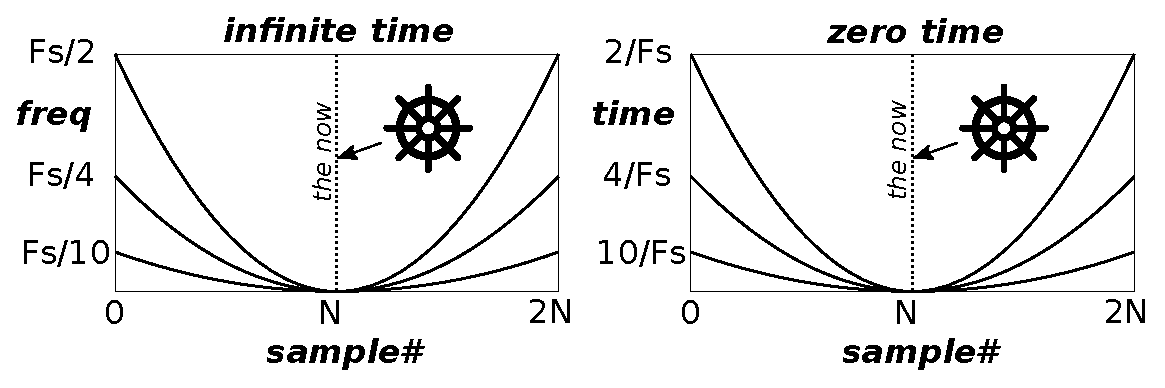
\includegraphics[width=0.95\linewidth]{../source/parabola_e}
    \caption[Hypothetical Parabolic Frequency Chirp]{Parabolic Chirp}
\end{figure}

\begin{equation} \label{eq:parabolic}
f(t, t_{now}) = k \cdot (t - t_{now})^2
\end{equation}

The singularity could have zero time instead of zero frequency:

\begin{equation} \label{eq:parabolictime}
f(t, t_{now}) = k / (t - t_{now})^2
\end{equation}

A problem with this model is that the cosine is periodic.
If signals were present, one would expect periodic artifacts that would have
been detected by now. Frequency analysis of electronic noise
from $10^{-6}$ Hz to over 1 THz can be found in the literature.
However, it's only a problem if the chirp is repeating in the same timeline.
The chirps could be on uncorrelated timelines in the multiverse.

A chirp would only be detectable if its timeline enters the realm of phenomena
that actually occur.
Considering outcomes as arising from probabilistic fields,
the most likely probabilities should produce the strongest signals.
Each chirp could be imagined as a conic section intersecting the light cone of
a Minkowski Space Time diagram. 
Whether the conic section is parabolic, hyperbolic or elliptical, within the 
system passband (which is assumed to be very limited) it looks parabolic.

Tests found that the signal was difficult to detect when it was more than 
10 dB below the noise.
Although it's an interesting possibility,
the low sensitivity of the conic section model doesn't engender much confidence
in its ability to model nature.

However, if the observer interacts through consciousness with what is being
observed, interfering signals could be worked around.
The system would compensate for them as a sort of forward error correction.
If the living system can detect the signal, perhaps the algorithm can too.
The sensor would have to interact with the living system to see what it sees.
Otherwise, the uncorrelated noise would swamp it.

\subsection{Information in the Noise}

Since chirps are bounded in time, a single chirp has a finite
existence within a practical bandwidth. 
It corresponds to a discrete impulse in the relative time domain,
or one symbol of information.
The idea of consciousness as time quanta may be useful here.
The act of being is a stream of consciousness that could have corresponding
streams of pulse-coded information, a kind of informational counterpart to DNA.
The impulse stream would be decoded for its information content.

To establish a notation and unit of measurement for quantum frequency,
let the ``warp factor'' $\omega$ be in units of $e$, the
mathematical constant derived by Leonhard Euler in the 1720s, per unit time.
The pronunciation may be ``e's per second'' for e/s, for example.

Note that 1.0 e/s is very close to twice the Golden Ratio $(\Phi=1.618:1)$,
so one should be careful when making assumptions about Golden Ratio relationships
in nature.

%%%%%%%%%%%%%%%%%%%%%%%%%%%%%%%%%%%%%%%%%%%%%%%%%%%%%%%%%%%%%%%%%%%%%%%%%%%%%%%%
\subsection{A Spiral Conceptual Model}

\begin{figure}[h]
    \centering
    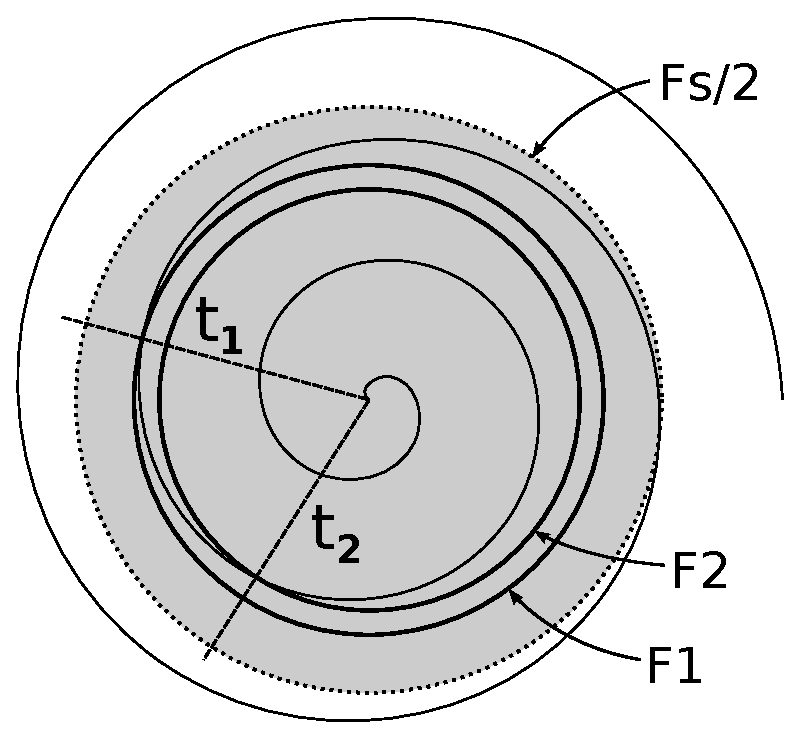
\includegraphics[width=0.7\linewidth]{../source/spiral_e}
    \caption[Quantum to Relative Time Relation]{Log polar plot of exponential chirp}
    \label{fig:spiral}
\end{figure}

Resonant signals in the quantum time domain could be re-mapped to relative time
and demodulated by correlating a series of fast Exponential Chirp Transforms (ECT). 
The spiral model needs $\omega$ to be real for Eq. \ref{eq:wp} to be self-similar.

The correlation effect can be visualized as a spinning logarithmic spiral
illuminated by a strobe light. When the strobe frequency matches the rate
constant of the spiral(s), it appears to be standing still.
Otherwise, it's a blur.

The relationship between quantum time and relative time can be thought of as a
2D plot in log-polar format.
Log-polar format renders a logarithmic spiral as a linear (Archimedean) spiral.
The spiral's radius is $\rho = k\theta$, where $k$ is a rate constant.
$\rho$ can represent either time or frequency by flipping the sign of $k$.
For purposes of signal processing, let $\rho$ represent log frequency and
$\theta$ relative time.

Log-polar mapping has proven useful in machine vision \cite{Bonmassar}
because it approximates the primate visual map \cite{Schwartz}.
Humans are visual thinkers, so their waking consciousness should map onto the
log-polar structure of quantum time signaling.

Fig.~\ref{fig:spiral} plots an exponential chirp in log-polar format.
A line can be drawn outward from the center of the spiral, crossing it at
multiple points.
The line rotates clockwise (in the case of downward chirp) at a step size
(from $t_1$ to $t_2$) corresponding to the oversampling rate.
For example, if the oversampling rate is 36 (each input value is used 36 times),
the step size is $10^{\circ}$.
Each angular sweep of the unit circle
(beginning and ending at line $t_1$ or $t_2$)
represents the input to a version of the Mellin transform called the
``Exponential Chirp Transform'' (ECT) \cite{Bonmassar}, which is
basically a Fourier Transform with time-warped input.

The transform's frequency domain output is along line $t_1$ or $t_2$ from
approximately $\rho$ = 0 to Fs/2, where Fs/2 (the Nyquist frequency)
is shown by the dashed circle.
The radius of the circle represents the approximate bandwidth of the system.
Not all of the circle is used: Anti-aliasing cuts off before Fs/2, while signal
near the center is too spread out to be useful.

The ECT time-warps the chirp signal, which represents a single ``quantum tone''.
In the $360^{\circ}$ sweep at line $t_1$,
the chirp is time-warped to a tone F1 in relative time.
A time $t_2-t_1$ later, at line $t_2$,
it's time-warped to a tone of frequency F2.
Time warping is exponential.
Note that ``exponential time warping'' is different from ``dynamic time
warping'', a popular means of pattern-matching mostly linear signals.

A convenient side effect of time warping is to transform interference
(periodic signals) into wide-band noise.
The usual frequency peaks of EEG and HRV are thus reduced.
Periodic signals could be notched out as needed by appropriate filters
to further reduce their interfering effect.

Being logarithmic, quantum time has the property of frequency going as
$-\tau$ rather than $1/t$.
To change between time and frequency, just flip the sign of the exponent.
Tones are mirror images of time.
Signal processing is more convenient in terms of frequency,
so that is the focus of this paper.

%%%%%%%%%%%%%%%%%%%%%%%%%%%%%%%%%%%%%%%%%%%%%%%%%%%%%%%%%%%%%%%%%%%%%%%%%%%%%%%%
\subsubsection{\label{sec:level1}The Spiral Transform}

The basic data flow of signal conversion from one time domain to another
$(\tau \leftrightarrow t)$ is shown in Fig.~\ref{fig:sled}.
The conversion algorithm slides along the input and output data streams,
forward in time.
Data is processed in overlapping chunks.
In other words, after a block of processing,
the sliding part of Fig.~\ref{fig:sled} shifts slightly to the right.
In proportion to the amount of shift,
new input stream is exposed and new output stream is sent out.
The I/O streams are low-bandwidth compared to the compute-intensive
processing block.

\begin{figure}
    \centering
    \includegraphics[width=0.95\linewidth]{../source/sled_e}
    \caption[Quantum to Relative Time Translation Flow]{Inter-domain data flow}
    \label{fig:sled}
\end{figure}

There are two use cases: demodulation and modulation.
For demodulation $(\tau \rightarrow t)$, the input stream is in the quantum
time domain and the output stream is in the relative time domain.
The input stream consists of real numbers. It gets exponentially time-warped
to convert chirps to tones and fed through a FFT (Fast Fourier Transform).
The FFT result is linearized with respect to the quantum domain by exponentially
warping it and accumulating it in a correlator to
include many instances of the same incoming chirp.

For modulation $(t \rightarrow \tau)$, the input stream is in the relative time
domain and the output stream is in the quantum time domain.
It's the demodulation process in reverse.
The usual use case is demodulation, so that will be the focus of the paper.

%%%%%%%%%%%%%%%%%%%%%%%%%%%%%%%%%%%%%%%%%%%%%%%%%%%%%%%%%%%%%%%%%%%%%%%%%%%%%%%%
\subsubsection{\label{sec:level1}The Parabolic Transform}

A spectrum analyzer for the parabolic model is simpler than one for the spiral model.
The frequency chirps shown in Fig. \ref{fig:parabolic} is time-warped by 
re-sampling so as to shift the frequencies up to their respective
$F_S/2$, $F_S/4$, and $F_S/10$. This is fed through a Fourier Transform to produce
a new column of pixels for each new slice of raw input data.

